\documentclass[12pt]{article}

% Layout.
\usepackage[top=1in, bottom=0.75in, left=1in, right=1in, headheight=1in, headsep=6pt]{geometry}

% Fonts.
\usepackage{mathptmx}
\usepackage[scaled=0.86]{helvet}
\renewcommand{\emph}[1]{\textsf{\textbf{#1}}}

% TiKZ.
\usepackage{tikz, pgfplots}
\usetikzlibrary{calc, positioning}

% Misc packages.
\usepackage{amsmath,amssymb,latexsym}
\usepackage{graphicx}
\usepackage{array}
\usepackage{xcolor}
\usepackage{multicol}
\usepackage{fancyhdr}
\pagestyle{fancy}
\usepackage{adjustbox}


% Misc.
\renewcommand{\d}{\displaystyle}
\newcommand{\ds}{\displaystyle}
\newcommand{\ul}[1]{\underline{#1}}
\def\bc{\begin{center}}
\def\ec{\end{center}}
\def\be{\begin{enumerate}}
\def\ee{\end{enumerate}}

\newcommand{\ans}[1][1in]{\rule{#1}{.5pt}}


\lhead{Math F113X: Quiz 6}
\rhead{October 24, 2025}

\begin{document}

\vspace{1cm}

\noindent \emph{Name:} \hrulefill \quad  score:\ans[1cm] \ / 10 \\


There are 10 points possible on this quiz. No aids (book, notes, etc.)
are permitted. You may use a non-programmable calculator.  \emph{Show all work and supporting calculations for full credit. Explain how you get your answers.}

\makeatletter
\newcommand{\Letter}[1]{\@Alph{#1}}
\makeatother

\newcommand{\pic}[1]{
\begin{tikzpicture}[vtx/.style ={draw, circle, inner sep = 2 pt}, lbl/.style={fill=white, inner sep = 2pt, }]
\node[vtx,] (a) at (0,0) {A};
\node[vtx,left = #1 of a] (b) {B};
\node[vtx,left = #1 of b] (c) {C};
\node[vtx,below = #1 of a] (d) {D};
\node[vtx,below = #1 of b] (e) {E};
\node[vtx,below = #1 of c] (f) {F};
\node[vtx,below = #1 of d] (g) {G};
\node[vtx,below = #1 of f] (h) {H};
\foreach \i/\j/\k in {a/b/1, b/c/4, a/d/11, b/e/1, a/e/5,c/e/3,f/e/4, e/d/4, e/h/9,g/h/4,e/g/12, f/h/8,c/f/2,d/g/9}{\draw (\i) -- node[lbl]{\k} (\j);}
\foreach \i/\j/\k in {a/c/2, c/h/3, g/a/2}{\draw (\i) to[bend right = 40] node[lbl]{\k} (\j);}
\end{tikzpicture}
}

\newcommand{\blankpic}[1]{
\begin{tikzpicture}[vtx/.style ={draw, circle, inner sep = 2 pt}, lbl/.style={fill=white, inner sep = 2pt, }]
\node[vtx,] (a) at (0,0) {A};
\node[vtx,left = #1 of a] (b) {B};
\node[vtx,left = #1 of b] (c) {C};
\node[vtx,below = #1 of a] (d) {D};
\node[vtx,below = #1 of b] (e) {E};
\node[vtx,below = #1 of c] (f) {F};
\node[vtx,below = #1 of d] (g) {G};
\node[vtx,below = #1 of f] (h) {H};
%\foreach \i/\j/\k in {a/b/1, b/c/4, a/d/5, b/e/1, a/e/5,c/e/6,f/e/1, e/d/7, e/h/12,g/h/1,e/g/5, f/h/8,c/f/2,d/g/9}{\draw (\i) -- node[lbl]{\k} (\j);}
\end{tikzpicture}
}

\be
\item (4 points) Consider the following graph:

\bigskip

\pic{1.5}

\bigskip

\fbox{Nearest Neighbor Algorithm (NNA)} 

From the present vertex, move to the nearest \emph{unvisited} vertex until all vertices are visited. Then close the circuit. Break ties by choosing the alphabetically earlier vertex.

Use the \emph{Nearest Neighbor Algorithm} starting at vertex $A$ to find a Hamiltonian circuit in the graph. Draw the circuit on the vertices below, including the weights on the edges, and determine the weight of the circuit.

\vspace{1cm}

\blankpic{1.5} \hfill circuit weight \ans

\newpage

\item (4 points) Here's the same graph from the front page, along with a table of edges sorted by weight.

\begin{adjustbox}{valign = t%, minipage{.4\linewidth}
}
\pic{1.3}
\end{adjustbox} \hspace{1cm} 
\begin{adjustbox}{valign = t%, minipage{.4\linewidth}
}
\begin{tabular}{c | c | c |}
edge & weight & used?\\ \hline
AB & 1 & \\
BE & 1 & \\
AC & 2 &\\
AG & 2 & \\
CF & 2 & \\
CE & 3 & \\
CH & 3 & \\
BC & 4 & \\
ED & 4 & \\
\end{tabular}
 \begin{tabular}{c | c | c}
 edge & weight & used?\\ \hline
EF & 4 & \\
GH & 4 & \\
AE & 5 & \\
 FH & 8 & \\
 DG & 9 & \\
 EH & 9 & \\
 AD & 11 & \\
 EG & 12 & \\
 &\\
 \end{tabular}
 \end{adjustbox}

\fbox{Cheapest Link Algorithm:} Select the cheapest edge in the graph that does not create a vertex of degree 3 or close the circuit too soon. Break ties by choosing edges that are ordered alphabetically earlier.

%\bigskip

Use the Cheapest Link Algorithm to find a Hamiltonian circuit in the graph. Draw the circuit, along with the weights, on the vertices below and determine the weight of the circuit. 

\bigskip

\blankpic{1.3} \hfill circuit weight \ans
\bigskip

\item (2 points) Find a Hamiltonian circuit using the Cheapest Link algorithm on the graph to the bottom right. 

\bigskip

What weight do you get? \ans

\bigskip

What does this example say about whether the Cheapest Link algorithm is guaranteed to give you an optimal Hamiltonian cycle? Explain your answer.

\hfill
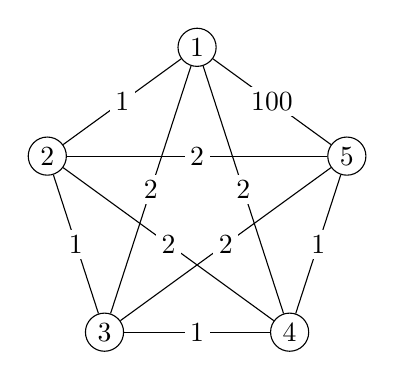
\begin{tikzpicture}[vtx/.style ={draw, circle, inner sep = 2 pt}, lbl/.style={fill=white, inner sep = 2pt}, scale = 2]
\foreach \i in {1,2,3,4,5}{\node[vtx] (\i) at (360/5*\i+18:1) {\i};}
\foreach \i/\j/\k in {1/2/1, 2/3/1,3/4/1
,4/5/1,5/1/100, 1/3/2,2/4/2,3/5/2,4/1/2,5/2/2
}{\draw (\i) --node[lbl]{\k} (\j);}
\end{tikzpicture}

\vfill

 \ee
\end{document}
%%% Local Variables:
%%% mode: LaTeX
%%% TeX-master: t
%%% End:
